\documentclass[aspectratio = 169]{chariteBeamer}
\usepackage[english]{babel} %% english
\usepackage[utf8]{inputenc}
\usepackage[T1]{fontenc}
\usepackage{hyperref}
\tikzset{>=latex}

\usepackage[edges]{forest}
\usetikzlibrary{positioning}
\usepackage{biostat}
\setbeamertemplate{caption}[numbered]
\let\qed\relax
\forestset{declare toks={elo}{}}
\graphicspath{{figures/}}
%% ================================================================== %% 

\author[L. Mödl, M. Becher, E. Sprünken]{Lukas Mödl, Matthias Becher, Erin Sprünken} 
\title{Day 2 -- Data and Statistics} 
\place{R-Course}
\date[]{Updated: \today}
\email{biometrie-rkurs@charite.de}

%% ================================================================== %% 

\hyphenation{Sam-ples}
\begin{document}



\begin{frame}[plain]
    \titlepage%
\end{frame}
\frame{\tableofcontents}



\section{Loading Data}
\begin{frame}[fragile]{Load}
  \begin{itemize}
	  \item \verb+ load() +
	  \item  \verb+ read.table() +
	  \item  \verb+ read.csv() +
  \end{itemize}
\end{frame}

\begin{frame}[fragile]{Options of read.csv()}
If we load CSV files in R, multiple parameters can be adjusted to tell R how the CSV is formatted. The most important parameters are:
  \begin{itemize}
	  \item \verb+header(TRUE/FALSE):+ Whether the first row contains variable names
	  \item \verb+sep:+ What symbol is used as a separator. Default is ",". Often ";" or "\textbackslash t"are used
	  \item \verb+dec:+ What is the decimal separator, i.e. do we use "." or "," for decimal places
	  \item	Example: \verb+read.csv("data.csv", header=TRUE, sep=";", dec=",")+
  \end{itemize}
\end{frame}

%% ================================================================== %%
\section{Indexing}
\begin{frame}[fragile]{Indexing}
	Often we only want certain elements of a vector, list or data.frame. There are multiple solutions to that. The most straightforward one is to use indices directly. Consider the following vector: \verb+ x <- c(1, 2, 3, 4, 5) +
	\begin{itemize}
		\item Choosing a certain value $\Leftrightarrow$ \verb+ x[1]+
		\item  Choosing multiple values $\Leftrightarrow$\verb+ x[c(1, 3, 5)]+
		\item  Choose multiple contiguous values $\Leftrightarrow$\verb+ x[1:3]+
		\item  Leave a certain value out $\Leftrightarrow$ \verb+x[-1]+
	\end{itemize}
\end{frame}

\begin{frame}[fragile]{Indexing of Lists and Data Frames}
	
	\begin{columns}[T]
	\begin{column}{0.5\textwidth}
List
		\begin{itemize}
		\item \verb+x[1]+
		\item \verb+x[[1]]+
	\end{itemize}
	\end{column}
	\begin{column}{0.5\textwidth}
Data Frame
	\begin{itemize}
		\item  \verb+x[1,]+
		\item  \verb+x[,1]+
		\item  \verb+x[,"Column1" ]+
		\item  \verb+x$Column1+
	\end{itemize}
	\end{column}
\end{columns}

\end{frame}

%% ================================================================== %%
\section{Descriptive Statistics}

\begin{frame}{Summary()}
	\begin{center}
		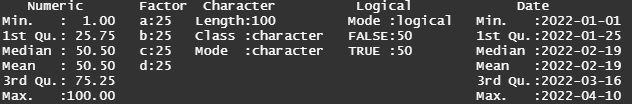
\includegraphics[scale=0.9]{Summary}
	\end{center}
\end{frame}

\begin{frame}[fragile]{Functions for Descriptive Statistics}
\begin{columns}[T]
	\begin{column}{0.5\textwidth}
		\begin{itemize}
			\item Mean = \verb+ mean() +
			\item Median = \verb+ median() +
			\item Minimum = \verb+ min() +
			\item Maximum = \verb+ max() +
			\item Standard Deviation = \verb+ sd() +
		\end{itemize}
	\end{column}
	\begin{column}{0.5\textwidth}
		\begin{itemize}
			\item Variance = \verb+ var() +
			\item Quantile = \verb+ quantile() +
			\item Correlation = \verb+ cor() +
			\item Covariance = \verb+ cov() +
			\item Contingency Table = \verb+ table() +
		\end{itemize}
	\end{column}
\end{columns}
Remark: sd() und var() divide by \verb+n-1+
\end{frame}

\begin{frame}[fragile]{Handling of NAs}
	When computing different statistics, NAs can pose a problem.\\
	\begin{itemize}
			\item Example: \verb+mean(c(1,2,3,4,5,NA))+ returns \verb+NA+\\
	\end{itemize}
	We solve this by providing \verb+na.rm = TRUE+ as an additional argument.\\
	\begin{itemize}
			\item Example: \verb+mean(c(1,2,3,4,5,NA), na.rm = TRUE)+ returns \verb+3+
	\end{itemize}
	The function \verb+is.na()+ detects whether there are NAs in a vector, data frame etc.
\end{frame}

%% ================================================================== %%
\section{Conversion and filtering}
\begin{frame}[fragile]{Conversion of Data}
	\begin{itemize}
		\item Numeric $\Leftrightarrow$ \verb+as.numeric()+
		\item Character $\Leftrightarrow$ \verb+as.character()+
		\item Factor $\Leftrightarrow$ \verb+as.factor()+
		\item Date $\Leftrightarrow$ \verb+as.Date()+
		\item Logical $\Leftrightarrow$ \verb+as.logical()+
	\end{itemize}
\end{frame}



\begin{frame}[fragile]{Filtering of Data}
Often, we want to filter our data regarding certain criteria, e.g. if we want to analyze only female subjects or only patients above a certain age. R provides different options to do so.
	\begin{itemize}
		\item  \verb+==+
		\begin{itemize}
			\item  \verb+data[data$Sex == "F",]+
		\end{itemize}
		\item  \verb+%in%+
		\begin{itemize}
			\item  \verb+data[data$Color %in% c("blue", "red"),]+
		\end{itemize}
		\item  \verb+subset()+
		\begin{itemize}
			\item  \verb+subset(data, Age < 50)+
		\end{itemize}
	\end{itemize}
\end{frame}

\begin{frame}[fragile]{Logical Operators}
If we want to check for multiple conditions at the same time, we can connect them with a logical operator instead of filtering one after another. R understands the following operators:\\
\begin{itemize}
			\item  and = \verb+&+
			\item  or (inclusive) = \verb+|+
			\item Not = \verb+!+
\end{itemize}
Furthermore, there are functions simplifying operations:\\
\begin{itemize}
			\item all(x) $\Leftrightarrow$ checks, whether a logical vector contains only \verb+TRUE+ 
			\item any(x) $\Leftrightarrow$ checks, whether a logical vector contains at least one \verb+TRUE+
			\item which(x) $\Leftrightarrow$ checks, at which positions a logical vector contains \verb+TRUE+
\end{itemize}
Example:
	\begin{itemize}
		\item  \verb+data[data$Sex != "M" & data$Age > 50,]+
	\end{itemize}
\end{frame}

%% ================================================================== %%

\section{Plots}

\begin{frame}[fragile]{Scatterplot}
	\begin{itemize}
		\item \verb+plot(data$Height, data$Weight)+
	\end{itemize}
			
	\begin{center}
		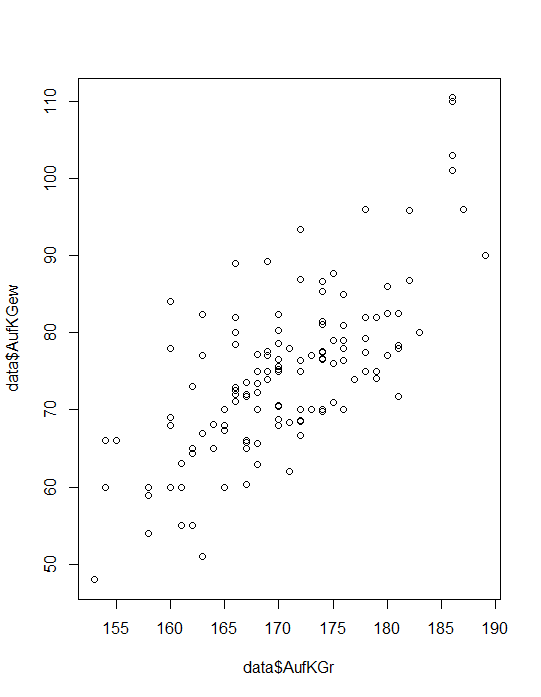
\includegraphics[height=6cm]{Scatterplot}
	\end{center}
\end{frame}

\begin{frame}[fragile]{Boxplot}
	\begin{itemize}
		\item \verb+boxplot(data$Sex == 0,]$Height, data[data$Sex == 1,]$Height)+
	\end{itemize}
			
	\begin{center}
		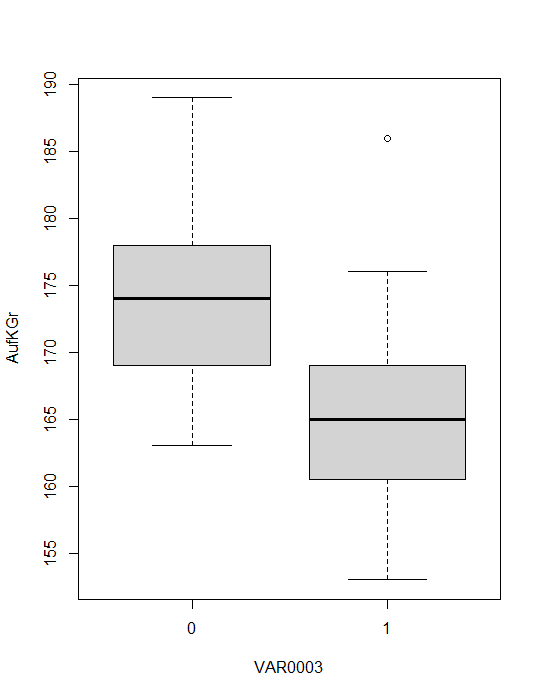
\includegraphics[height=6.5cm]{Boxplot}
	\end{center}
\end{frame}

\begin{frame}[fragile]{Histogram}
	\begin{itemize}
		\item \verb+hist(data$Weight)+
	\end{itemize}
			
	\begin{center}
		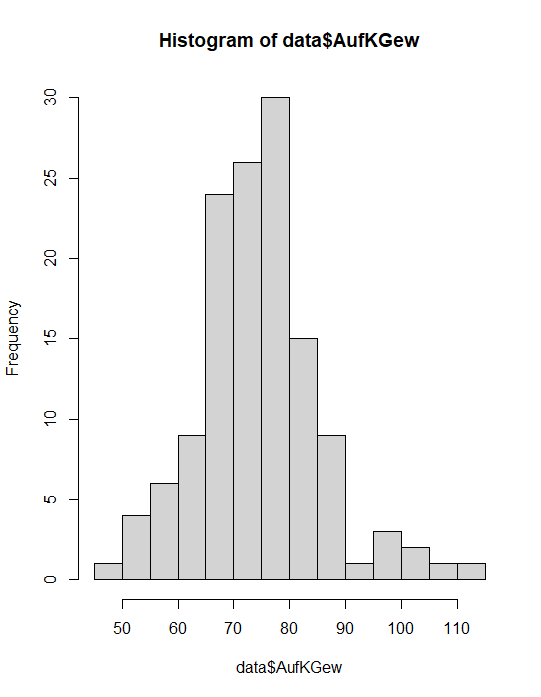
\includegraphics[height=6.5cm]{Histogram}
	\end{center}
\end{frame}

\begin{frame}[fragile]{Histogram with Density}
	\begin{itemize}
		\item \verb+hist(data$Weight, probability = T) + \\ \verb+lines(density(data$Weight))+
	\end{itemize}
			
	\begin{center}
		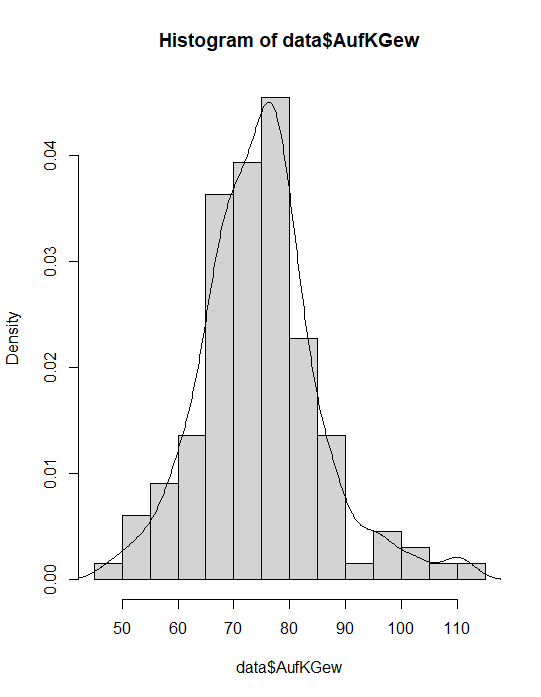
\includegraphics[height=6cm]{Density}
	\end{center}
\end{frame}

\begin{frame}[fragile]{Barplot}
	\begin{itemize}
		\item \verb+ barplot(summary(as.factor(data$Klinik)))+
	\end{itemize}
			
	\begin{center}
		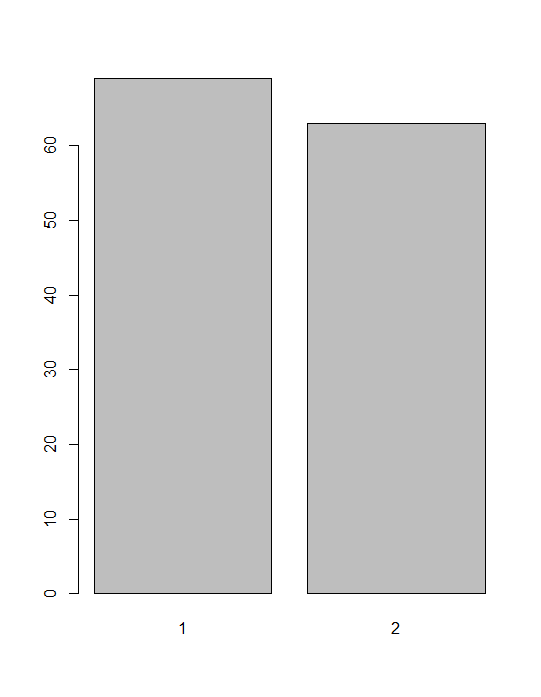
\includegraphics[height=6.5cm]{Barplot}
	\end{center}
\end{frame}

\begin{frame}[fragile]{Kaplan-Meier Plot}
	\begin{itemize}
		\item \verb+library(survival)+ \\ \verb+data_vet <- veteran+ \\ \verb+km_fit <- survfit(Surv(time, status) ~ 1, data=data_vet)+ \\ \verb+plot(km_fit)+
	\end{itemize}
			
	\begin{center}
		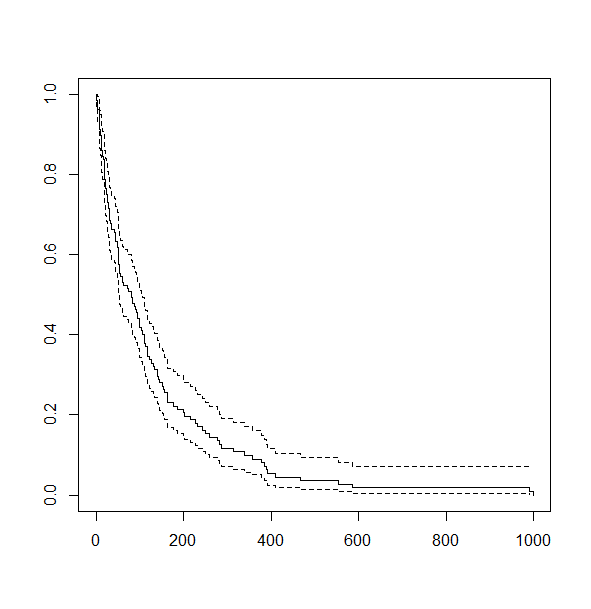
\includegraphics[height=5cm]{KM1}
	\end{center}
\end{frame}

\begin{frame}[fragile]{Kaplan-Meier Plot}
	\begin{itemize}
		\item \verb+library(survminer)+ \\ \verb+ggsurvplot(km_fit)+
	\end{itemize}
			
	\begin{center}
		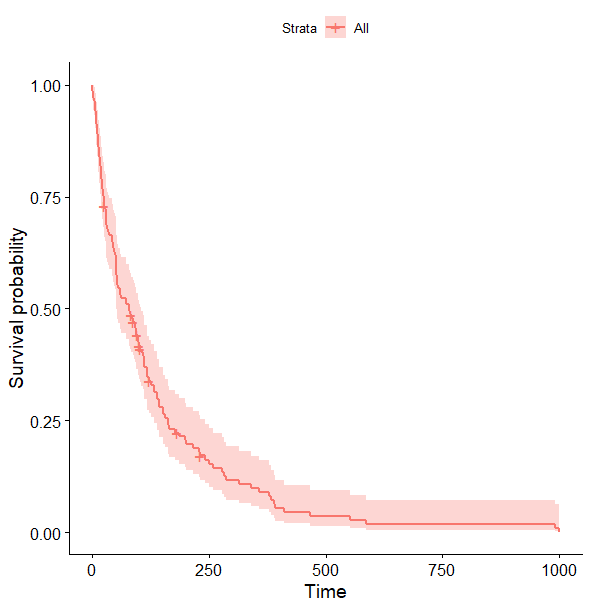
\includegraphics[height=5.5cm]{KM2}
	\end{center}
\end{frame}

\begin{frame}[fragile]{Kaplan-Meier Plot}
	\begin{itemize}
		\item \verb+km_fit <- survfit(Surv(time, status) ~ trt, data=data_vet)+ \\ \verb+ggsurvplot(km_fit)+
	\end{itemize}
			
	\begin{center}
		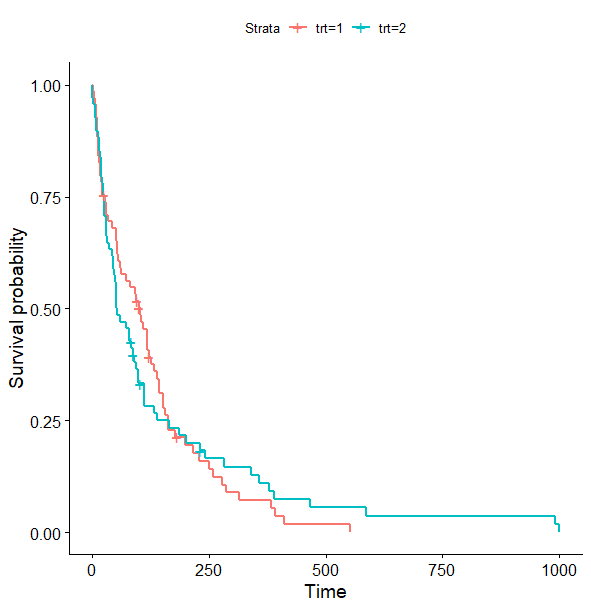
\includegraphics[height=5.5cm]{KM3}
	\end{center}
\end{frame}

\begin{frame}[fragile]{Labels for Plots}
	Plots are very flexibel and can be adjusted in many different ways. For example, we can include axis labels and a title.
	\begin{itemize}
		\item Beispiel: \verb+plot(data$Height, data$Weight, xlab="Größe,"+
		\verb+            ylab="Gewicht", main="Scatterplot")+
	\end{itemize}
			
	\begin{center}
		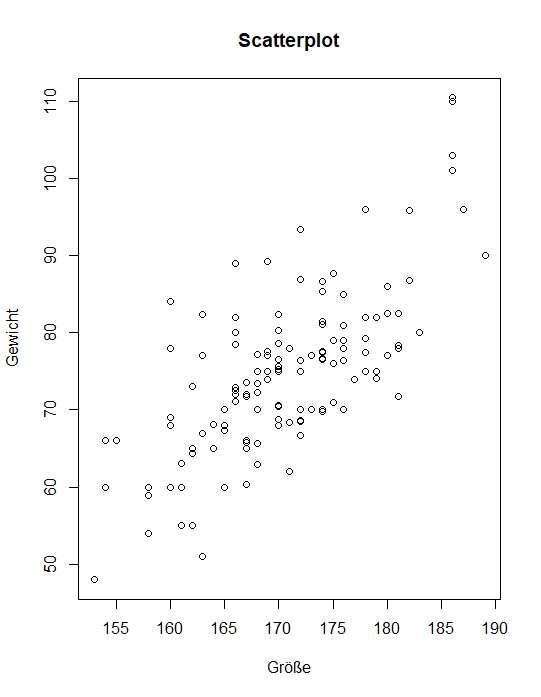
\includegraphics[height=4.5cm]{AnnotatedPlot}
	\end{center}
\end{frame}

\begin{frame}[fragile]{Saving of Plots}
	\begin{columns}[T]
		\begin{column}{0.5\textwidth}
			\begin{center}
				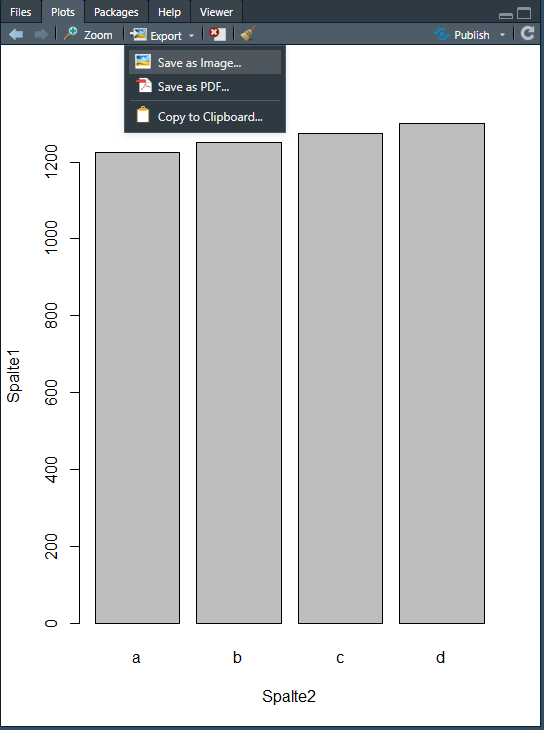
\includegraphics[height=5.5cm]{SaveImage}
			\end{center}
		\end{column}
		\begin{column}{0.5\textwidth}
			\begin{center}
				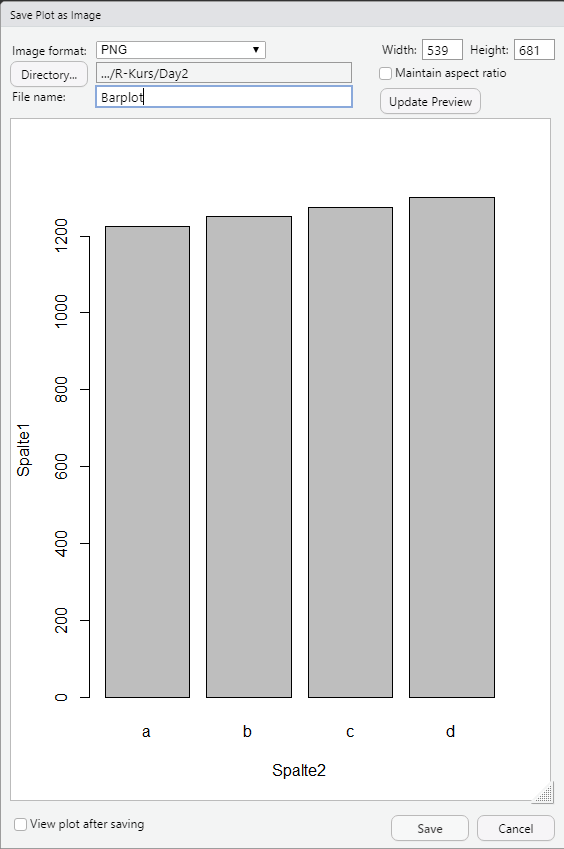
\includegraphics[height=5.5cm]{SaveImage2}
			\end{center}
		\end{column}
	\end{columns}	
\end{frame}

\end{document}
%% ================================================================== %%
%% ================================================================== %% 
